\DocumentMetadata{
 lang=en,
   pdfversion=2.0,
   pdfstandard=ua-2,
   uncompress,
   pdfstandard=a-4f,
   testphase = {phase-III,math,title}}
 % \tagpdfsetup{math/mathml/write-dummy}
 
\documentclass[a4paper,12pt,twoside]{article}
\renewcommand{\familydefault}{\sfdefault}

%% Define a compact list environment
\newenvironment{itemize*}%
  {\begin{itemize}%
    \setlength{\itemsep}{0pt}%
    \setlength{\parskip}{0pt}}%
  {\end{itemize}}


%%%%%%%%%%%%%%%%%%%%%%%%%%%%%%%%%%%%%%%%%%%%%%%%%%
%%%      Specify whether exam, resit/delayed 1st sit or coursetest     %%%%%%
%%%%%%%%%%%%%%%%%%%%%%%%%%%%%%%%%%%%%%%%%%%%%%%%%%

\newcount\ctype
\ctype=2	%   1    for Main Series UG Examination,  
 		%   2    for ALL  Resit/Delayed First Sit, 
             	%   3    for Coursetest
              	%   4    for Delayed  First Sit Main Series UG Examination,  
%% See phyexam.sty for definitions of \ctype options.

%%%%%%%%%%%%%%%%%%%%%%%%%%%%%%%%%%%%%%%%%%%%%%%%%%%
\usepackage{graphicx,amsmath,amsfonts,ifthen,calc, phyexam, latexsym, amssymb}
\hypersetup{pdftitle=MODULE TITLE EXAM}
\usepackage[mathscr]{euscript}
\usepackage{pdfcomment}  % Use to insert alt-text for figures as tooltips
\pagestyle{exambody}
\ExplSyntaxOn
\makeatletter
\pdfxform_new:nnn {tooltip/AP}{}
  { { \opacity_select:n{0}\rule{\paperwidth}{\paperheight} }}
\pdf_object_new:n {tooltip/AP}
\pdf_object_write:nne {tooltip/AP}{dict}{/N <</Yes~\pdfxform_ref:n{tooltip/AP}~/Off~\pdfxform_ref:n{tooltip/AP}>>}
\renewcommand{\pc@annot@tooltip}%
{%
  /TU~(\pc@pdfenc@contents)\space%
  /Contents~(\pc@pdfenc@contents)\space%<<<<<<<<<<<<
  /T~(tooltip \thezref@unique)\space%
  /C~[ ]\space%
  /FT/Btn\space%
  /F~516\space% Print=true + ToggleNoView = false instead of 768
  /Ff~65536\space%
  /H/N\space%
  /BS~<< /W~0 >>\space%
  /AP~\pdf_object_ref:n{tooltip/AP}
}
\ExplSyntaxOff
\makeatother


%%%%%%%%%%%%%%%%%%%%%%%%%%%%%%%%%%%%%%%%%%%%%%%%%%%
%%%  Specify Academic Session. This must be in the format 201X--1X+1
%%%%%%%%%%%%%%%%%%%%%%%%%%%%%%%%%%%%%%%%%%%%%%%%%%%
 
\renewcommand{\cyear}{2021-2}  
 
%%%%%%%%%%%%%%%%%%%%%%%%%%%%%%%%%%%%%%%%%%%%%%%%%%%
%%%     Set Course Title, Code, Rubric, Time
%%%     Choose one of the rubrics.
%%%     State Author or Paper Coordinator
%%%     Set Version Number, default =1  or as advised by Examinations Office.
%%%%%%%%%%%%%%%%%%%%%%%%%%%%%%%%%%%%%%%%%%%%%%%%%%%

\newcommand{\ctitle}{MODULE TITLE}
\newcommand{\ccode}{PHY-XXXXY}
\newcommand{\crubricone}{
\textbf{Timings}\\
This examination paper will be available for 24 hours, from 9:30AM UK time.\\
It is recommended you spend a maximum of \textbf{2 hours} completing this examination. 
Students entitled to Assessment Adjustments: You should apply any
extra or rest break time to which you are entitled in addition, up to the maximum 24-hour limit.\\\\
\textbf{Instructions}\\
Answer \textbf{ANY THREE out of the four questions}\\\\
You are advised to spend an equal amount of time on each question.\\
The breakdown of marks within each question is indicated by the percentage figures in square brackets on the right.\\\\
\textbf{Word count}\\
No question in this assessment has a maximum word count. You are expected to include concise and clear explanations in your working. No question requires prose answers beyond brief sentences.\\\\
\textbf{Additional materials}\\
There are no additional materials for this paper.
}
\newcommand{\crubrictwo}{
\textbf{Academic Integrity}\\
To maintain academic integrity students are required:
\begin{itemize*}
\item Not to keep an electronic copy of this paper or share the content with others.
\item To ensure that all work produced is solely their own. Students are
  advised that their work will be checked using text matching software
  to determine any similarity with the work of other students or with
  other published materials.
\item To be aware that the University policy regarding plagiarism and
  collusion will apply to this examination.
  \href{https://www.uea.ac.uk/about/university-information/university-governance/academic-calendar/section-3/general-regulations/university-policy-on-plagiarism-and-collusion}{You
  can view the policy here}.
\end{itemize*}
\textbf{Submission}
\begin{itemize*}
\item The submission point for this examination will close at 9:30AM
  UK time, 24 hours after being made available. It is recommended that you submit your exam script as soon as completed.
\item All answers must be submitted as a \textbf{SINGLE} Word or pdf
  document (and you \textbf{MUST} include your student number in the file name), unless otherwise instructed.
\item Guidance on submitting un-typed answers, such as diagrams and
  graphs, can be found on Blackboard, below this paper.
\end{itemize*}
} 

\newcommand{\ctime}{2 Hours}
\newcommand{\cauthor}{Dr Module Organiser, PHY}
\newcommand{\cversion}{Version 1}

%\cpnumbersetting THIS APPLIES ONLY TO CONCESSION PAPERS, NO CHANGE OTHERWISE.
%\newcommand{\cpnumber}{1000354672}    %concession paper student registration number, blank out if needed.
\newcommand{\cpnumber}{\phantom{XXXXXXX}} %concession paper student registration umber 

%%%%%%%%%%%%%%%%%%%%%%%%%%%%%%%%%%%%%%%%%%%%%%%%%%%
%%%       Put your own macros here      %%%%%%%%%%%
%%%%%%%%%%%%%%%%%%%%%%%%%%%%%%%%%%%%%%%%%%%%%%%%%%%

%\newcommand{\CC}{{\mathcal C}}
%\newcommand{\Cl}{{\mathscr Cl}}
%\newcommand{\la}{{\langle}}
%\newcommand{\ra}{{\rangle}}
%\newcommand{\Aut}{{\rm Aut}}
%\newcommand{\s}{{\sigma}}
%\newcommand{\bv}{{\boldsymbol v}}
%\newcommand{\C}{{\mathbb C}}
\newcommand{\Q}{{\mathbb Q}}
%\newcommand{\R}{{\mathbb R}}
\newcommand{\Z}{{\mathbb Z}}
%\newcommand{\F}{{\mathbb F}}
%\newcommand{\om}{{\omega}}
%\newcommand{\ga}{\alpha}
%\newcommand{\gb}{\beta}
%\newcommand{\gs}{\sigma}
%\newcommand{\Di}{\mbox{ \large$\mid$ }} 
%\newcommand{\dm}{{\rm dim}}
%\newcommand{\re}{I\!\!R}  
%\newcommand{\gl}{\lambda}
%\newcommand{\gm}{\mu}
%\newcommand{\abs}[1]{\left|#1\right|}  %absolute value
%\newcommand{\N}{{\mathbb N}}
%\newcommand{\e}{{\rm e}}
%\renewcommand{\i}{{\rm i}}
%\newcommand{\bomega}{\mbox{\boldmath ${\omega}$ }}
%\newcommand{\bOmega}{\mbox{\boldmath ${\Omega}$}}
%\newcommand{\btau}{\mbox{\boldmath ${\tau}$}}
%\newcommand{\eo}{\epsilon_0}

\def\grad{\mbox{\boldmath $\nabla$}}
\renewcommand{\div}[1]{\grad\cdot #1}
\newcommand{\divr}[1]{\grad_{\r}\cdot #1}
%\newcommand{\grad}[1]{\nabla #1}
\newcommand{\curl}[1]{\grad\times #1}

\renewcommand{\v}[1]{\ensuremath{\mathbf{#1}}}
\def\mc#1{{\mathcal #1}}
\def\emptyline{\vspace{12pt}}
\newcommand{\pd}[2]{\frac{\partial #1}{\partial #2}}
\newcommand{\pds}[2]{\frac{\partial^2 #1}{\partial #2^2}}
\newcommand{\tpd}[2]{\frac{\textrm{d}#1}{\textrm{d}#2}}
\newcommand{\tpds}[2]{\frac{\textrm{d}^2 #1}{\textrm{d} #2^2}}
\newcommand{\E}{\v{E}}
\newcommand{\B}{\v{B}}
\newcommand{\M}{\v{M}}
\renewcommand{\H}{\v{H}}
\newcommand{\J}{\v{J}}
\newcommand{\F}{\v{F}}
%\newcommand{\vv}{\v{v}}
\newcommand{\A}{\v{A}}
\newcommand{\D}{\v{D}}
\renewcommand{\P}{\v{P}}
\renewcommand{\r}{\v{r}}
\renewcommand{\d}{\v{d}}
\newcommand{\er}{\epsilon_r}
\newcommand{\hr}{\hat{\r}}
\newcommand{\dr}{\v{dr}}
%\newcommand{\dd}{\textrm{d}}
\def\dd{\mbox{d}}
\newcommand{\n}{\v{n}}
\newcommand{\hp}{\hat\phi}
\newcommand{\x}{{\bf\widehat x}}
\newcommand{\y}{{\bf\widehat y}}
\newcommand{\z}{{\bf\widehat z}}
\newcommand{\eo}{\epsilon_0}
\newcommand{\gr}{\nabla}
\newcommand{\cu}{\nabla\times}
\newcommand{\di}{\nabla\cdot}
\newcommand{\lap}{\nabla^2}
\newcommand{\R}{\mathbb R}
\newcommand{\C}{\mathbb C}
\newcommand{\T}{\mathbb T}
%\renewcommand{\i}{\v{i}}
%\renewcommand{\j}{\v{j}}
%\renewcommand{\k}{\v{k}}
\newcommand{\0}{\v{0}}
%\newcommand{\e}{{\rm e}}
\newcommand{\hf}[1]{\widehat f(#1)}
\newcommand{\hg}[1]{\widehat g(#1)}
\newcommand{\hh}[1]{\widehat h(#1)}
\renewcommand{\(}{\left(}
\renewcommand{\)}{\right)}
%\newcommand{\thalf}{{\textstyle{\frac{1}{2}}}}
\newcommand{\im}{\text{i}}
\newcommand{\nhat}{\ensuremath{\v{\hat{n}}}}
\newcommand{\xhat}{\ensuremath{\v{\hat{x}}}}
\newcommand{\yhat}{\ensuremath{\v{\hat{y}}}}

\newcommand{\vv}[1]{\mathbf{#1}}
\newcommand{\vi}{\mathbf{i}}
\newcommand{\vj}{\mathbf{j}}
\newcommand{\vx}{\mathbf{{\widehat x}}}
\newcommand{\vy}{\mathbf{{\widehat y}}}\newcommand{\dtheta}{{\dot\theta}}
\newcommand{\thalf}{\textstyle{\frac{1}{2}}}
\newcommand{\dq}{\dot q}
\newcommand{\s}{\mathbf{s}}

\newcommand{\e}{{\rm e}}
\renewcommand{\i}{{\rm i}}
   % Put user-defined commands in this file and uncomment.

%%%%%%%%%%%%%%%%%%%%%%%%%%%%%%%%%%%%%%%%%%%%%%%%%%%
%%%                  Document starts         %%%%%%
%%%%%%%%%%%%%%%%%%%%%%%%%%%%%%%%%%%%%%%%%%%%%%%%%%%

\begin{document}
\titlep
%\baselineskip=22pt  % Not used.

% %%%%%%%%%%%%%%%%%%%%%%%%%%%%%%%%%%%%%%%%%%%%%%%%%%%
% %%%%%%             General instructions to candidates (if required)
% %%%%%%%%%%%%%%%%%%%%%%%%%%%%%%%%%%%%%%%%%%%%%%%%%%%

% Not used


%%%%%%%%%%%%%%%%%%%%%%%%%%%%%%%%%%%%%%%%%%%%%%%%%%%%%
%%%%%              Begin exam proper          %%%%%%%
%%%%%%%%%%%%%%%%%%%%%%%%%%%%%%%%%%%%%%%%%%%%%%%%%%%%%

%\begin{center}
% \textbf{PART I}\\  %Uncomment if dividing exam into parts
Answer \emph{THREE} of the questions 1--4
%\end{center}
  
\questionsbegin  % This begins enumerating the questions 


%%%%%%%%%%%%%%%%%%%%%%%%%%%%%%%%%%%%%%%%%%%%%%%%%%%%%%
%%%%                   Question 1                 %%%%
%%%%%%%%%%%%%%%%%%%%%%%%%%%%%%%%%%%%%%%%%%%%%%%%%%%%%%

\item
  Answer \emph{all} parts (a)--(c) % Instructions can be put here
  \qitemsbegin %If different parts of the question are in different files, put \qitemsbegin outside
  \item
The first part of Question 1 needs a couple of equations
\begin{eqnarray*}
\vv{r}_1&=& \ldots,
\\
\vv{r}_2&=&\ldots,
\end{eqnarray*}
followed by some more text.

Finally the tast and the corresponding number of marks
\mmark{15}

\item
Part (b) of Question 1 is divided into subparts
\qqitemsbegin
\item
Show that \ldots

\item
Show that \ldots

\item
Finally compare \ldots and mark given only for (b) as a whole, not each subpart separately.\\
\mmark{35}
\qqitemsend

  ~\\
\centerline{\pdftooltip{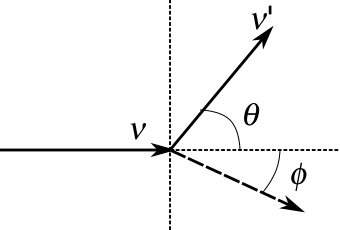
\includegraphics[width=0.3\textwidth,alt=
Photon of frequency nu incident horizontally from left on stationary electron. The photon scatters upwards with frequency nu-prime at angle theta with the horizontal. The electron scatters downwards at angle phi with the horizontal.
]{compton.png}}{Photon of frequency nu incident horizontally from left on stationary electron. The photon scatters upwards with frequency nu-prime at angle theta with the horizontal. The electron scatters downwards at angle phi with the horizontal.}}
Part (c) of Question 1 makes use of a figure, including a tooltip for accessibility. The question ends with an equation, in which the marks are indicated.
Show that
\begin{equation*}
  \tan\phi = \ldots,
  \mtag{50}
\end{equation*}

  \qitemsend
  \clearpage  %Use clearpage if needed to begin next question on a new page

%%%%%%%%%%%%%%%%%%%%%%%%%%%%%%%%%%%%%%%%%%%%%%%%%%%%%%
%%%%                   Question 2                 %%%%
%%%%%%%%%%%%%%%%%%%%%%%%%%%%%%%%%%%%%%%%%%%%%%%%%%%%%%

\item 
  Answer \emph{all} parts (a)--(c)
  \qitemsbegin
\item For Question 2, only one input file is used and contains all commands for the different parts and subparts. 

This is part (a), which again has an eqation. Show that
  \begin{equation*}
    \frac{\partial L}{\partial q_i} = \ldots \mtag{40}
  \end{equation*}
\item Part (b) is entirely explained by text. \mmark{20}

\item Part (c) requires both inline equations $T=\ldots$ and some equations asking the student to show that
  \qqitemsbegin
  \item This equation
    \begin{equation*}
      \frac{\partial L}{\partial q} = \ldots,
    \end{equation*}
    \vspace{-12pt}
  \item And also these simulataneous equations
    \begin{equation*}
      \frac{dp}{dt} = \ldots, \qquad \frac{dq}{dt} = \ldots.
    \end{equation*}
    \mmark{40}
  \qqitemsend
\qitemsend

%\questionsend  %If dividing into several parts, put a \questionsend command at the end of each part

\clearpage

%% Unomment and modify as needed to begin the next part:
%\begin{center}
%  \textbf{PART II}\\
%Answer \emph{EITHER} Question 3 \emph{OR} Question 4
%\end{center}

% Reset qnum if exam broken into parts, necessitating interrupting \questionsbegin ... \questionsend:
%\questionsbegin \setcounter{qnum}{2}

%%%%%%%%%%%%%%%%%%%%%%%%%%%%%%%%%%%%%%%%%%%%%%%%%%%%%%
%%%%                   Question 3                 %%%%
%%%%%%%%%%%%%%%%%%%%%%%%%%%%%%%%%%%%%%%%%%%%%%%%%%%%%%

\item 
  Answer \emph{all} parts (a)--(c)
  And Question (3) continues in the same manner, but has no clearpage following. \mmark{100}

%\clearpage

%%%%%%%%%%%%%%%%%%%%%%%%%%%%%%%%%%%%%%%%%%%%%%%%%%%%%%
%%%%                   Question 4                 %%%%
%%%%%%%%%%%%%%%%%%%%%%%%%%%%%%%%%%%%%%%%%%%%%%%%%%%%%%

\item Answer \emph{both} parts (a) and (b)

Question 4 has all instructions and commands included in the input file.
\qitemsbegin
\item One part \mmark{50}
\item And the other. \mmark{50}
\qitemsend


%%%%%%%%%%%%%%%%%%%%%%%%%%%%%%%%%%%%%%%%%%%%%%%%%%%%%%
%%%%                  END OF PAPER                %%%%
%%%%%%%%%%%%%%%%%%%%%%%%%%%%%%%%%%%%%%%%%%%%%%%%%%%%%%
\begin{center}   \bf END OF PAPER  \end{center}  \vfill
\thispagestyle{end}
\questionsend

\end{document} 
